\chapter{Plano de Gerenciamento de Requisitos}
\label{gerency}

\section{Introdução}

A finalidade deste documento é documentar como será a rastreabilidade dos requisitos, bem como quais atributos serão utilizados para classificar os mesmos. Desta forma os requisitos estarão sendo analisados, documentados e gerenciados durante todo o ciclo de vida do projeto.

\section{Gerenciamento de Requisitos}

\subsection{Organização, Responsabilidades e Interfaces}

De forma geral, não há uma distribuição de responsabilidade dentre os integrantes do time para ser o responsável pelo projeto EnGerir, no âmbito de que restringir a execução e documentação das atividades deste projeto. Mas há membros responsáveis pela completude de determinadas tarefas.

\subsection{ Ferramentas, Ambiente e Infra-Estrutura}

Dentre as ferramentas utilizadas no desenvolvimento do projeto, encontram-se:

\begin{itemize}
\item Google Docs: como um ambiente compartilhado para a documentação de boa parte dos artefatos gerados pelo processo escolhido.
\item Innoslate: como ferramente escolhida para o gerenciamento dos requisitos do projeto.
\item Bizagi: como ferramenta para modelar o processo.
\item Astah: como ferramenta de produção do diagrama de caso de uso.
\end{itemize}

\section{Programa de Gerenciamento de Requisitos}

\subsection{Identificação dos Requisitos}

\begin{table}[h!]
\centering
\caption{Identificação dos Requisitos}
\label{identification}
\begin{tabular}{|p{4cm}|p{4cm}|p{4cm}|}
\hline
Artefato(Tipo de Documento)             & Item de Rastreabilidade         & Descrição                                                                                \\ \hline
Documento de Visão                      & Necessidade dos Envolvidos(NE)  & Descrição das principais necessidades dos stakeholders, bem como seus devidos atributos. \\ \hline
Documento de Visão                      & Características(CA)             & Descrição das características                                                            \\ \hline
Especificação de Caso de Uso            & Regras de negócio(RN)           & Descrição das regras de negocio a serem atendidas nos casos de uso.                      \\ \hline
Especificação de Requisitos de Software & Requisitos funcionais(RF)       & Descrição dos requisitos elicitados, bem como os seus devidos atributos.                 \\ \hline
Especificação Suplementar               & Requisitos não funcionais (RNF) & Descrição dos requisitos não funcionais elicitados, bem como os seus devidos atributos.  \\ \hline
Modelo de Casos de Uso                  & Casos de Uso(UC)                & Descrição dos casos de uso e seus respectivos disgramas.                                 \\ \hline
\end{tabular}
\end{table}

\clearpage{}

\subsection{Rastreabilidade}

\begin{figure}[htb]
	\centering
	\label{rastreabilidade2}
		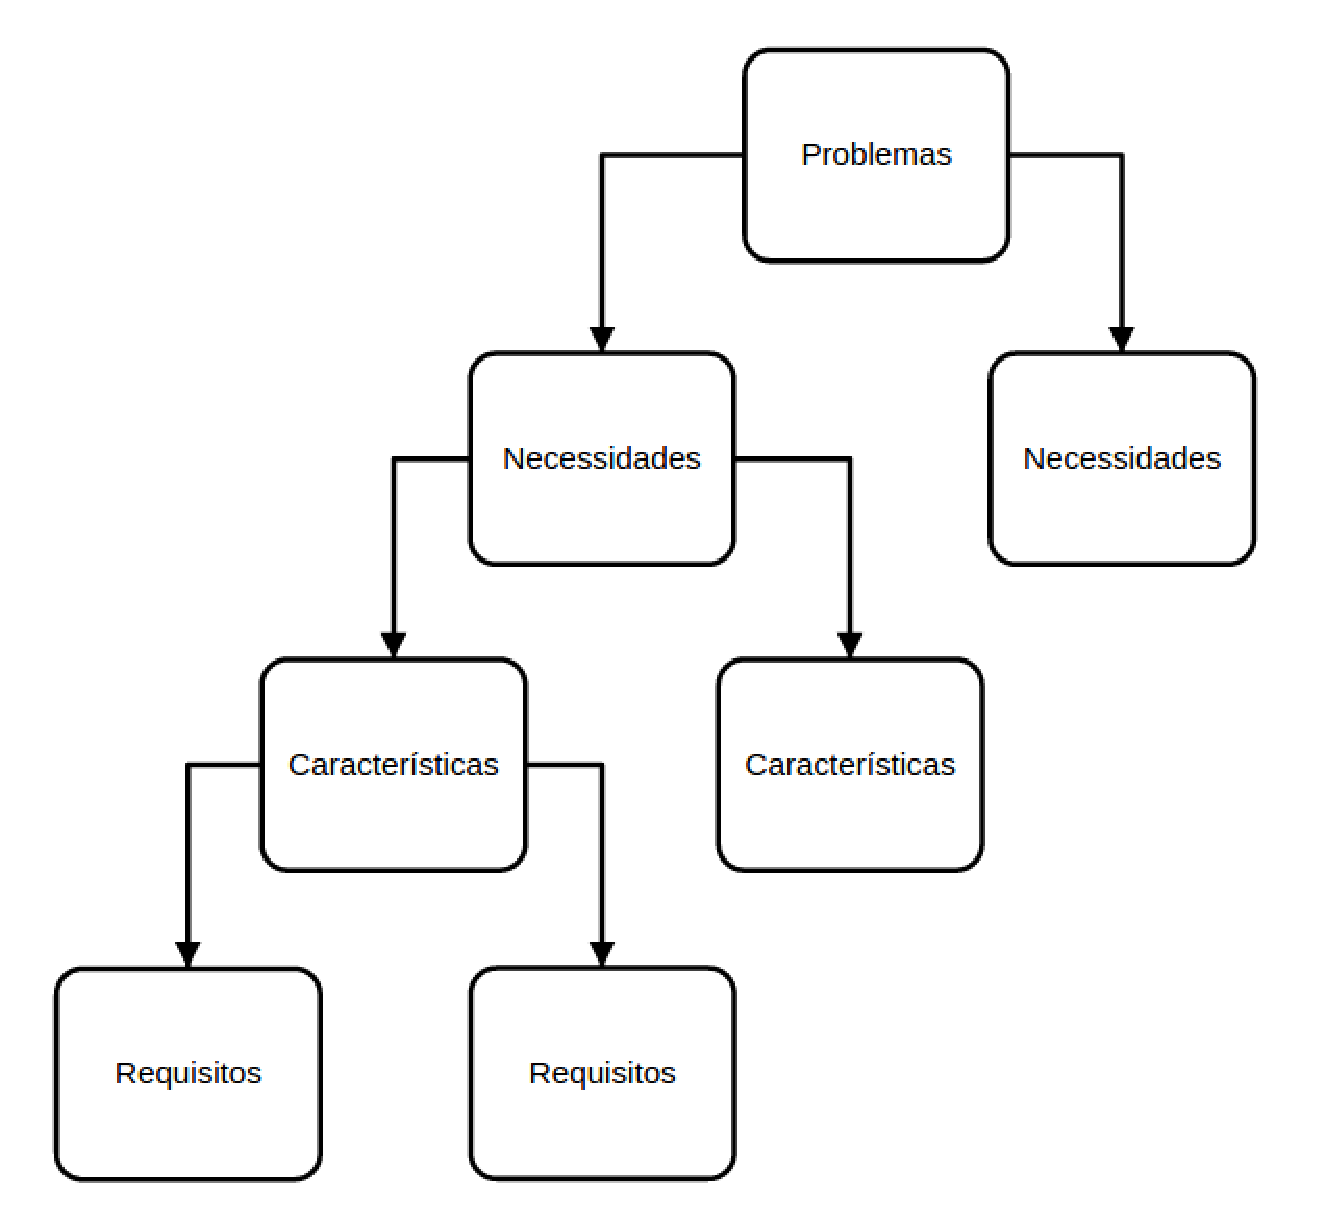
\includegraphics[keepaspectratio=true,scale=0.6]{figuras/rastreabilidade2.eps}
	\caption{Rastreabilidade adotada}
\end{figure}

\clearpage{}

\subsection{Atributos}

De modo geral, todos os nossos itens de rastreabilidade seguem os mesmos atributos, sendo eles:

\begin{itemize}
\item Prioridade;
\item Status;
\item Dificuldade;
\end{itemize}

\subsubsection{Prioridade}

Define o quão importante é o requisito para o sistema em relação aos demais. Os de maior prioridade serão implementados o quanto antes.

\begin{description}
\item [Alta] Sinaliza que este requisito é de extrema importância para o sistema e deve ser implementado o quanto antes.
\item [Média] Sinaliza que este requisito embora importante ele pode ter a sua implementação postergada em favor de um requisito de alta prioridade.
\item [Baixa] Um requisito que com a mais baixa prioridade ficará mais para o final do desenvolvimento do sistema ou quando outros requisitos mais importantes já estivem completos.
\end{description}

\subsubsection{Status}

Define o andamento de um determinado requisito durante o desenvolvimento do sistema.

\begin{description}
\item [Não inicializado] Usado para sinalizar que o item em questão ainda não foi inicializado, no sentido de que por algum requerimento, como depender de outros itens já terem sido finalizados, este teve o seu desenvolvimento postergado.
\item [Em andamento] Sinaliza que este item está sendo desenvolvido.
\item [Completado] Sinaliza que este item já foi concluído.
\end{description}

\subsubsection{Dificuldade}

Serve de indicativo para uma possível dificuldade na implementação dos requisitos. É um atributo fundamental para o planejamento das iterações.

\begin{description}
\item [Alta] Um requisito com um alto este nível de dificuldade receberá uma maior atenção em relação aos demais, pois este pode influenciar fortemente no desenvolvimento do sistema.
\item [Média] Um requisito com este nível não representa um grande risco para a implementação dos sistema.
\item [Baixa] Sinaliza que este requisito pode ser facilmente implementado sem maiores riscos ou agravantes.
\end{description}

\subsection{Gerenciamento de Mudança de Requisitos}

\subsubsection{Processamento e Aprovação de Solicitações de Mudança}

De acordo com o nosso processo de \textit{software}, as aprovações e mudanças serão sempre feitas em concordância com os \textit{stakeholders} e em etapas bem definidas do processo.

\subsubsection{Comitê de Controle de Mudança (CCB)}

Havendo uma concordância entre um representante dos \textit{stakeholders} e os membros do grupo de desenvolvimento, já é considerado como uma mudança válida.

\subsubsection{Fluxos de Trabalho e Atividades}

Embora qualquer membro do grupo de desenvolvimento do projeto possa estar trabalhando em um determinado requisito, sempre haverá um membro responsável por este, para garantir a completude do mesmo.


\subsubsection{Matriz de rastreabilidade}

Para um melhor entendimento da hierarquia do requisitos elicitados, foram descritas algumas matrizes de rastreabilidade contendo:

\begin{itemize}
  \item{Problemas X Necessidades}
  \item{Necessidades X Características}
  \item{Características X Requisitos}
\end{itemize}


% Problemas X Necessidades

\begin{table}[!h]
\centering
\caption{Problemas X Necessidades}
\label{Problemas_X_Necessidades_1}
\begin{tabular}{|c|c|c|c|}
\hline
  & \multicolumn{3}{c|}{\textbf{Necessidades}} \\ \hline
    \multirow{2}{*}{\textbf{Problemas}} &             & NE 1.1        & NA 1.2       \\ \cline{2-4}
                                        & PB 1        & X             & X            \\ \hline
\end{tabular}
\end{table}

% Necessidades X Características

\begin{table}[!h]
\centering
\caption{Necessidades X Características}
\label{Necessidades_X_Caracteristicas_1}
\begin{tabular}{|c|c|c|c|c|c|}
\hline
  & \multicolumn{5}{c|}{\textbf{Características}}      \\ \hline
    \multirow{2}{*}{\textbf{Necessidades}} &        & CA 1.1.1 & CA 1.1.2 & CA 1.2.1 & CA 1.2.2 \\ \cline{2-6}
                                                    & NE 1.1 & X        & X        &          &          \\ \cline{2-6}
                                                    & NE 1.2 &          &          & X        & X        \\ \hline
\end{tabular}
\end{table}


\begin{table}[!h]
\centering
\caption{Necessidades X Características}
\label{Necessidades_X_Caracteristicas_2}
\begin{tabular}{|c|c|c|}
\hline
  & \multicolumn{2}{c|}{\textbf{Características}} \\ \hline
    \multirow{3}{*}{\textbf{Necessidades}} &  & CA 1.2.3               \\ \cline{2-3}
                                              & NE 1.1               &                        \\ \cline{2-3}
                                              & NE 1.2               & X                      \\ \hline
\end{tabular}
\end{table}


% Características X Requisitos

\begin{table}[!h]
\centering
\caption{Características X Requisitos}
\label{Características_X_Requisitos_1}
\begin{tabular}{|c|c|c|c|c|c|}
\hline
  & \multicolumn{5}{c|}{\textbf{Requisitos}}                    \\ \hline
    \multirow{6}{*}{\textbf{Características}} &   & RF 1.1.1.1 & RF 1.1.1.2 & RF 1.1.1.3 & RF 1.1.1.4 \\ \cline{2-6}
                                       & CA 1.1.1 & X          & X          & X          & X         \\ \cline{2-6}
                                       & CA 1.1.2 &            &            &            &           \\ \cline{2-6}
                                       & CA 1.2.1 &            &            &            &           \\ \cline{2-6}
                                       & CA 1.2.2 &            &            &            &           \\ \cline{2-6}
                                       & CA 1.2.3 &            &            &            &           \\ \hline
\end{tabular}
\end{table}


\begin{table}[!h]
\centering
\caption{Características X Requisitos}
\label{Características_X_Requisitos_2}
\begin{tabular}{|c|c|c|c|c|c|}
\hline
  & \multicolumn{5}{c|}{\textbf{Requisitos}}                    \\ \hline
    \multirow{6}{*}{\textbf{Características}} &   & RF 1.1.1.5 & RF 1.1.1.6 & RF 1.1.1.7 & RF 1.1.1.8 \\ \cline{2-6}
                                       & CA 1.1.1 & X          & X          & X          & X         \\ \cline{2-6}
                                       & CA 1.1.2 &            &            &            &           \\ \cline{2-6}
                                       & CA 1.2.1 &            &            &            &           \\ \cline{2-6}
                                       & CA 1.2.2 &            &            &            &           \\ \cline{2-6}
                                       & CA 1.2.3 &            &            &            &           \\ \hline
\end{tabular}
\end{table}


\begin{table}[!h]
\centering
\caption{Características X Requisitos}
\label{Características_X_Requisitos_3}
\begin{tabular}{|c|c|c|c|c|c|}
\hline
  & \multicolumn{5}{c|}{\textbf{Requisitos}}                    \\ \hline
    \multirow{6}{*}{\textbf{Características}} &   & RF 1.1.2.1 & RF 1.1.2.2 & RF 1.1.2.3 & RF 1.2.1.1 \\ \cline{2-6}
                                       & CA 1.1.1 &            &            &            &           \\ \cline{2-6}
                                       & CA 1.1.2 & X          & X          & X          &           \\ \cline{2-6}
                                       & CA 1.2.1 &            &            &            &  X        \\ \cline{2-6}
                                       & CA 1.2.2 &            &            &            &           \\ \cline{2-6}
                                       & CA 1.2.3 &            &            &            &           \\ \hline
\end{tabular}
\end{table}


\begin{table}[!h]
\centering
\caption{Características X Requisitos}
\label{Características_X_Requisitos_4}
\begin{tabular}{|c|c|c|c|c|c|}
\hline
  & \multicolumn{5}{c|}{\textbf{Requisitos}}                    \\ \hline
    \multirow{6}{*}{\textbf{Características}} &   & RF 1.2.1.2 & RF 1.2.1.3 & RF 1.2.1.4 & RF 1.2.1.5 \\ \cline{2-6}
                                       & CA 1.1.1 &            &            &            &           \\ \cline{2-6}
                                       & CA 1.1.2 &            &            &            &           \\ \cline{2-6}
                                       & CA 1.2.1 & X          & X          & X          &  X        \\ \cline{2-6}
                                       & CA 1.2.2 &            &            &            &           \\ \cline{2-6}
                                       & CA 1.2.3 &            &            &            &           \\ \hline
\end{tabular}
\end{table}


\begin{table}[!h]
\centering
\caption{Características X Requisitos}
\label{Características_X_Requisitos_5}
\begin{tabular}{|c|c|c|c|c|c|}
\hline
  & \multicolumn{5}{c|}{\textbf{Requisitos}}                    \\ \hline
    \multirow{6}{*}{\textbf{Características}} &   & RF 1.2.1.6 & RF 1.2.2.1 & RF 1.2.2.2 & RF 1.2.3.1 \\ \cline{2-6}
                                       & CA 1.1.1 &            &            &            &           \\ \cline{2-6}
                                       & CA 1.1.2 &            &            &            &           \\ \cline{2-6}
                                       & CA 1.2.1 & X          &            &            &           \\ \cline{2-6}
                                       & CA 1.2.2 &            & X          & X          &           \\ \cline{2-6}
                                       & CA 1.2.3 &            &            &            & X         \\ \hline
\end{tabular}
\end{table}


\begin{table}[!h]
\centering
\caption{Características X Requisitos}
\label{Características_X_Requisitos_6}
\begin{tabular}{|c|c|c|c|c|}
\hline
  & \multicolumn{4}{c|}{\textbf{Requisitos}}                    \\ \hline
    \multirow{6}{*}{\textbf{Características}} &   & RF 1.2.3.2 & RF 1.2.3.3 & RF 1.2.3.4 \\ \cline{2-5}
                                       & CA 1.1.1 &            &            &            \\ \cline{2-5}
                                       & CA 1.1.2 &            &            &            \\ \cline{2-5}
                                       & CA 1.2.1 &            &            &            \\ \cline{2-5}
                                       & CA 1.2.2 &            &            &            \\ \cline{2-5}
                                       & CA 1.2.3 & X          & X          & X          \\ \hline
\end{tabular}
\end{table}




